\documentclass{midl} % Include author names

% The following packages will be automatically loaded:
% jmlr, amsmath, amssymb, natbib, graphicx, url, algorithm2e
% ifoddpage, relsize and probably more

% Header for extended abstracts
\jmlrproceedings{MIDL}{Medical Imaging with Deep Learning}
\jmlrpages{}
\jmlryear{2026}

\jmlrworkshop{Short Paper -- MIDL 2026 submission}
\jmlrvolume{-- Under Review}
\editors{Under Review for MIDL 2026}

\title[MRI-derived Face Age vs Brain Age]{MRI-derived Face Age vs Brain Age from the Same T1 Scan: a Longitudinal Single-Subject Stress Test}

\midlauthor{%
  \Name{Ekaterina Kondrateva\nametag{$^{1}$}} \orcid{0000-0003-3623-6106} \Email{ekaterina.kondrateva@maastrichtuniversity.nl}\\
  \Name{Ramil Khafizov\nametag{$^{2}$}}\\
  \Name{Gleb Bobrovskikh\nametag{$^{2}$}}\\
  \addr $^{1}$ Department of Radiation Oncology (Maastro), GROW Research Institute for Oncology and Reproduction, Maastricht University Medical Centre+, Maastricht University, Maastricht, The Netherlands\\
  \addr $^{2}$ Applied AI Institute
}

\begin{document}

\maketitle

\begin{abstract}
  A non-defaced T1-weighted MRI carries both a brain and a facial surface,
  but off-the-shelf age models are pretrained on cohorts that may not
  overlap with the test subject.  We run SynthBA (brain age, trained on
  $4{,}105$ subjects with a bimodal age distribution peaking at $25$ and
  $74$~yr) and two face-age methods---multi-view renders scored by FaceAge
  (trained on $56{,}304$ photographs of subjects aged $\geq 60$~yr) and
  BioFace3D-20 morphometrics---on the SIMON longitudinal single-subject
  dataset ($99$ scans, $36$ scanners, ages $29$--$46$~yr).
  %
  SynthBA predicts $27.4 \pm 1.26$~yr across all scans (MAE $16.2$~yr): the
  SIMON age window sits in the valley of SynthBA's bimodal training
  distribution, and the model regresses toward the nearest training mode
  ($25$~yr).  The prediction is biased but not blind: slope against
  chronological age is $+0.148$~yr/yr ($p<10^{-4}$), so $\sim 15\%$ of the
  true aging rate survives.  Neither face method tracks aging in this
  subject (morphometrics slope $+0.04$, $p{=}0.84$; FaceAge slope
  $-0.14$, $p{=}0.44$); FaceAge additionally carries a $+8.5$~yr bias
  inherited from its $\geq 60$~yr training cohort.
  %
  When a brain-age model is reproducible across $36$ scanners (SD
  $1.26$~yr) but biased by $16$~yr, the failure is training-distribution
  geometry rather than scanner noise or preprocessing.
\end{abstract}

\begin{keywords}
  brain age, face age, MRI, longitudinal, reproducibility, out-of-distribution, SIMON
\end{keywords}

% -----------------------------------------------------------------------
\section{Introduction}
% -----------------------------------------------------------------------

Standard MRI pre-processing pipelines routinely remove facial structure
(``defacing'') to protect participant identity before data sharing.
However, non-defaced T1-weighted volumes still contain both a brain and a
complete facial surface within the same acquisition.  This makes it possible
to estimate two age signals from one file and ask whether they behave
similarly under repeated scanning.

Prior work on brain age~\citep{peng2021sfcn, puglisi2024synthba} and face
age~\citep{bontempi2025faceage} usually treats these as separate modalities
acquired by different instruments.  A same-scan comparison removes that
acquisition mismatch, and a longitudinal single-subject dataset adds a stricter
test: can a model follow aging within one person rather than merely produce
scanner-stable predictions?

More broadly, biological-age estimation may become useful for earlier disease
detection or risk stratification, not only for age prediction itself.  For
example, FaceAge suggested that face-derived biological age carries clinically
relevant signal beyond chronological age in oncology~\citep{bontempi2025faceage}.

We use the SIMON dataset~\citep{duchesne2019simon}, which contains 99 T1 scans of one
healthy subject acquired across 36 scanners while he ages from 29 to 46
years, as a controlled stress test.  Our goals are: (1) run face-age and
brain-age estimation on the same T1 volume; and (2) measure whether each
branch tracks longitudinal aging or collapses to a reproducible but incorrect
age estimate.

% -----------------------------------------------------------------------
\section{Methods}
% -----------------------------------------------------------------------

\paragraph{Face branch.}
Given a T1 NIfTI volume, we extract the iso-surface with marching cubes
(intensity threshold $t{=}30$) and render the face with PyVista~\citep{pyvista}
from nine viewpoints ($\pm 20^\circ$ yaw/pitch) under randomized lighting.
We evaluate two face estimators.  First, we apply
FaceAge~\citep{bontempi2025faceage}, a ResNet-50 model trained on 56\,304
curated photographs, to each render and average the predictions.  Second,
we extract BioFace3D-20 landmarks from the multi-view renders, compute
GPA+EDMA morphometric features, and regress age with Ridge regression.
Because this paper focuses on SIMON as a stress test, we report raw
predictions and do not apply IXI-derived calibration.  Figure~\ref{fig:simon}A
shows a synthetic example of the MRI-derived multi-view render grid used as
input to the face branch.

\paragraph{Brain branch.}
Skull stripping is performed with SynthStrip~\citep{synthstrip}.  We then
run SynthBA~\citep{puglisi2024synthba}, a segmentation-based model designed
to be robust to acquisition variability, on the stripped volume.

\paragraph{Training data of the borrowed models.}
Both age models are used as pretrained black boxes; SIMON sits far from
both training distributions, which we make explicit here because it
shapes the interpretation of every result.  SynthBA was trained on
$4{,}105$ healthy subjects aggregated from ADNI, AIBL, IXI, HCP, and CoRR
($7{,}060$ T1w MRIs), spanning ages $6$--$95$ with a \emph{bimodal}
distribution peaking at $25$ and $74$~yr~\citep{puglisi2024synthba}.  The
SIMON $29$--$46$~yr window therefore lies in the trough between the two
training peaks.  FaceAge was trained on $56{,}304$ IMDb--Wiki photographs
of presumed-healthy individuals aged $\geq 60$~yr, deliberately curated to
match a clinical-oncology target population~\citep{bontempi2025faceage};
the SIMON subject is $14$--$30$~yr younger than the entire training
cohort.  We use both models without finetuning or recalibration by
design: the goal here is to characterise how off-the-shelf age models
behave on a same-scan longitudinal stress test, not to retrain them.

\paragraph{Dataset and evaluation setting.}
The \textbf{SIMON} dataset~\citep{duchesne2019simon} provides 99 T1 scans of a single
healthy male collected across 73 sessions on 36 scanners (age range
29.6--46.4 years).  Because identity is fixed, between-scan spread reflects
scanner sensitivity rather than subject heterogeneity, while the slope of
predictions over time provides a direct readout of longitudinal validity.

% -----------------------------------------------------------------------
\section{Results}
% -----------------------------------------------------------------------

Figure~\ref{fig:simon} plots chronological age against predicted age for all
three methods.  Three patterns stand out.

To quantify longitudinal tracking beyond visual inspection, we fit a
linear regression $\hat{y} = a\,y_{\text{chron}} + b$ for each method.
A slope $a{\to}1$ indicates faithful tracking of the subject's aging
(even if biased in mean); $a{\to}0$ indicates a frozen predictor.

\textbf{SynthBA (brain)} produces a nearly flat response: mean predicted
age $27.4 \pm 1.26$ years across all 99 scans despite the subject aging
from approximately $30$ to $46$ years (MAE $16.2$ yr, bias $-16.2$ yr).
The regression slope is nevertheless $+0.148$ per year
($\mathrm{SE}{=}0.036$, $p{=}6.9\times 10^{-5}$, $R^{2}{=}0.15$): about
$15\%$ of the true aging rate is recovered, so the brain parenchyma
changes are detectable even in this out-of-distribution regime, albeit
buried under an enormous constant offset.

\textbf{Face morphometrics} (GPA+EDMA features, Ridge regression) show a
positive bias of $+5.1$ yr and a spread of SD $5.6$ yr, but \emph{no
statistically detectable longitudinal trend}: slope $+0.038$ per year
($p{=}0.84$, $R^{2}{=}0.001$).  The scatter visible in
Figure~\ref{fig:simon}~B is driven by scanner and session variance at
each time point, not by within-subject aging.

\textbf{FaceAge multi-view renders} show the largest bias ($+8.5$ yr,
SD $5.7$ yr) and the widest scatter; the slope is negative and
non-significant ($-0.14$, $p{=}0.44$), consistent with the domain gap
between MRI surface renders and the photographic training distribution
of the model.

Neither face method tracks aging in this subject.  SynthBA, despite
appearing visually frozen, carries a statistically significant residual
longitudinal signal.

\begin{figure}[htbp]
\floatconts{fig:simon}
  {\caption{(A) Synthetic example of the MRI-derived multi-view face render
    grid used as input to the face branch. (B) Chronological vs predicted age
    on SIMON (one subject, 36 scanners, 99 scans). Dashed line: perfect
    prediction. Dotted horizontal lines: mean predicted age per method.
    SynthBA predicts a near-constant age regardless of the subject's actual
    age at scan (MAE $16.2$ yr, bias $-16.2$ yr), yet still shows a weak but
    statistically significant slope ($+0.148$, $p{<}10^{-4}$). Neither face
    method tracks aging longitudinally (morphometrics slope $+0.04$,
    $p{=}0.84$; FaceAge slope $-0.14$, $p{=}0.44$).}}
  {\begin{minipage}[t]{0.5\linewidth}
    \centering
    \textbf{A}\\[2pt]
    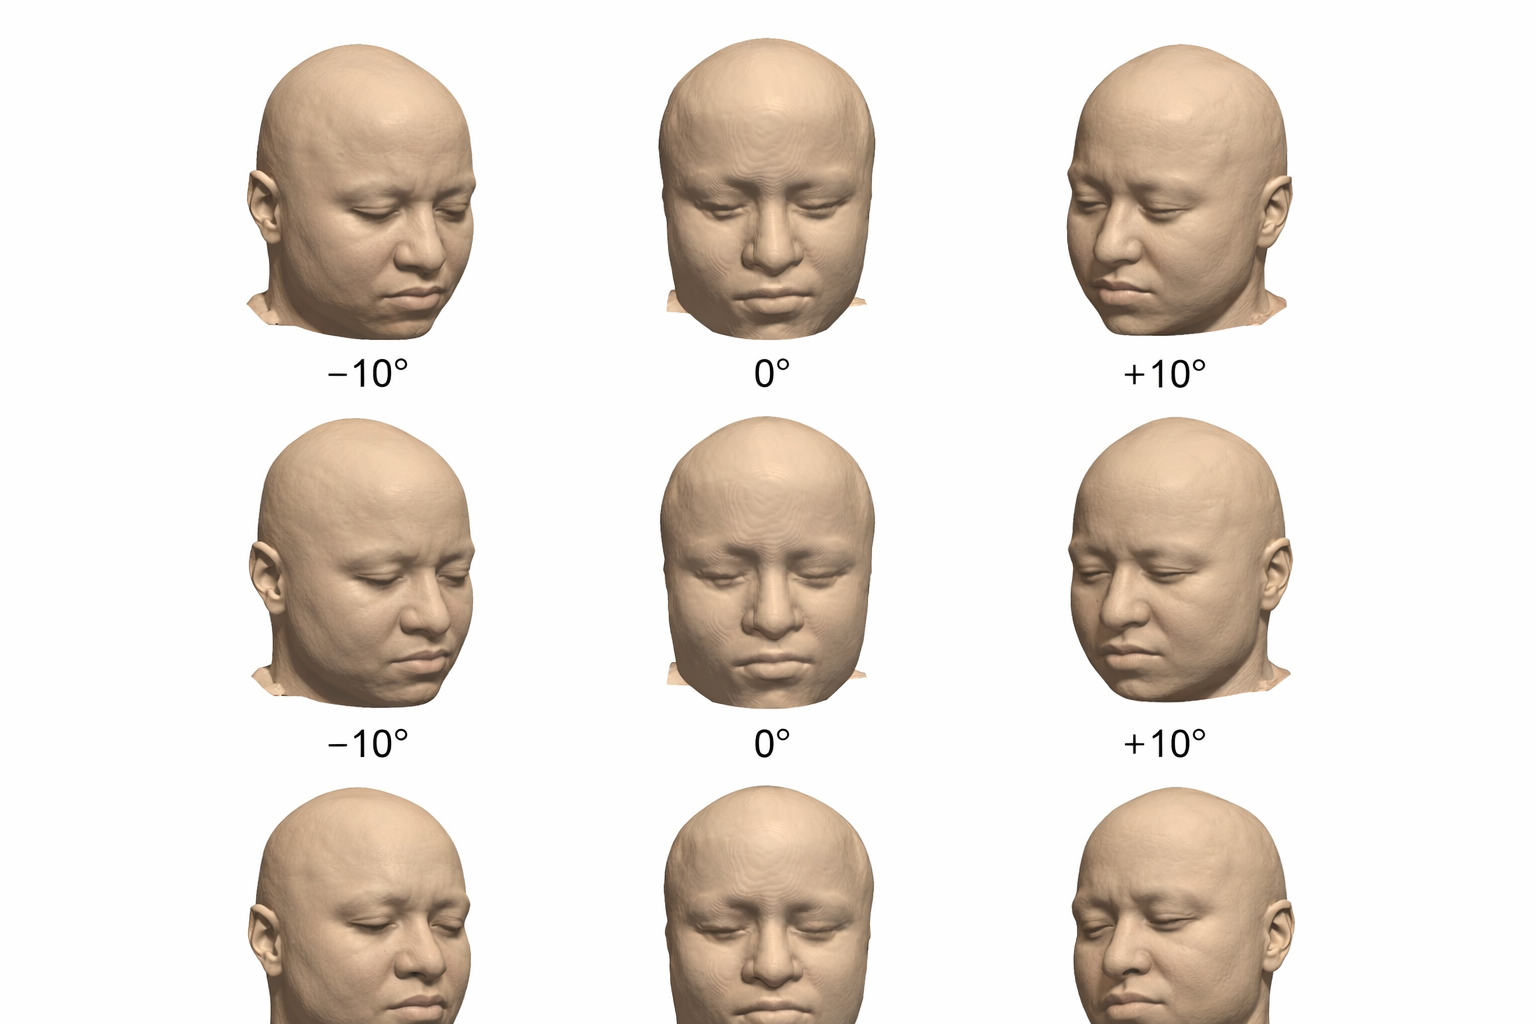
\includegraphics[width=\linewidth]{ex_render.png}
   \end{minipage}\hfill
   \begin{minipage}[t]{0.5\linewidth}
    \centering
    \textbf{B}\\[2pt]
    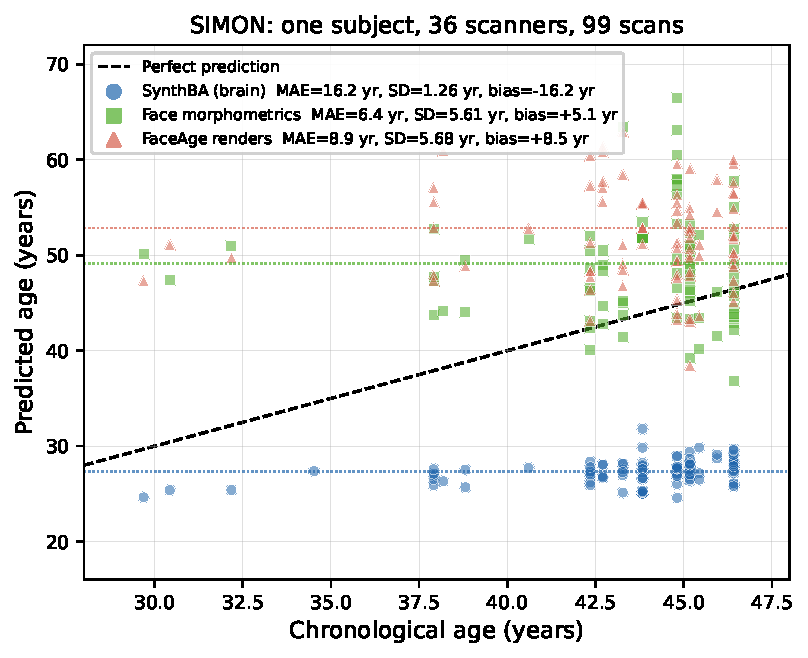
\includegraphics[width=\linewidth]{simon_chron_vs_predicted.pdf}
   \end{minipage}}
\end{figure}

\begin{figure}[htbp]
\floatconts{fig:training_dist}
  {\caption{SynthBA training-distribution geometry versus SIMON predictions.
    Coloured curves: per-dataset Gaussian approximations of the five
    cohorts that contributed to SynthBA training (HCP $n{=}1105$, CoRR
    $n{=}1461$, IXI $n{=}563$, ADNI $n{=}784$, AIBL $n{=}192$;
    per-dataset $N$ from Table I of \citet{puglisi2024synthba}, $\mu$ and
    $\sigma$ approximated from each cohort's publicly reported age
    statistics).  Gray fill: the weighted sum of the five components,
    bimodal with peaks near $29$ and $74$~yr, consistent with the
    bimodal training distribution Puglisi et al. report textually.
    Light-blue band: SIMON chronological-age range ($29.6$--$46.4$~yr),
    which sits in the trough between the two training modes.  Blue
    histogram: SynthBA predictions on the $99$ SIMON scans, clustering
    at the nearest training mode ($\sim 27$~yr) rather than within the
    SIMON age band.  The failure mode is geometric: the model has very
    little training mass in the SIMON age window.}}
  {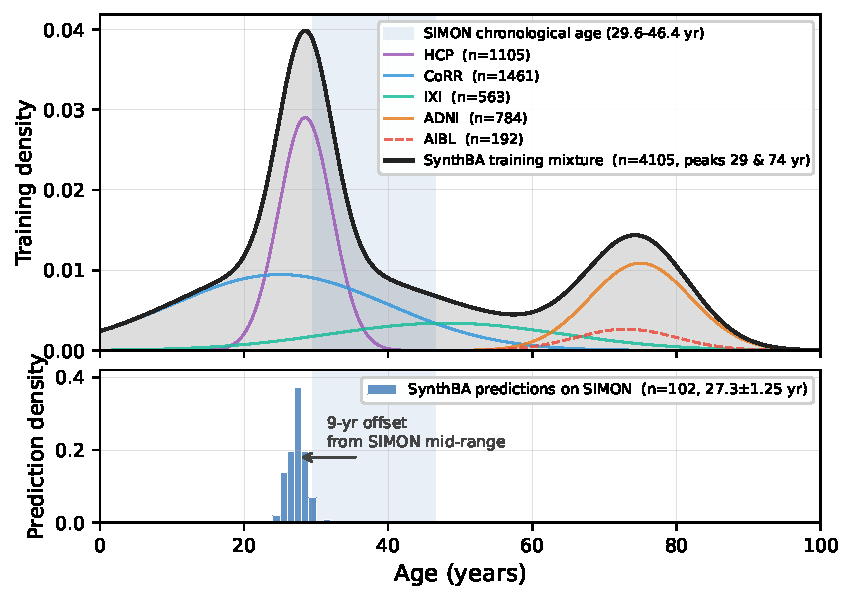
\includegraphics[width=0.95\linewidth]{synthba_training_vs_predictions.pdf}}
\end{figure}

\section{Discussion and Conclusion}

A non-defaced T1 MRI still contains two age-sensitive anatomical signals,
but the SIMON stress test shows that extracting them reliably is harder than
running pretrained models on the same file.  The main lesson is that low
scanner variance can mask severe biological error: SynthBA is reproducible
across hardware yet fails to follow the subject's aging trajectory.

Both face branches fail longitudinally in this subject.  FaceAge is
strongly biased on MRI surface renders (bias $+8.5$ yr) and its slope is
negative and non-significant, consistent with the photo-to-MRI domain
gap.  The morphometric branch is more calibrated in mean (bias $+5.1$
yr) but shows no significant longitudinal slope ($p{=}0.84$): the
visible spread in Figure~\ref{fig:simon}~B is scanner and session
variance, not aging.  Counter-intuitively, SynthBA --- which looks
visually frozen --- is the only method whose predictions track the
subject's aging at a detectable rate, recovering roughly $15\%$ of the
true slope.  This suggests that the longitudinal aging signal in T1 MRI
lives primarily in the parenchyma rather than in the facial surface as
captured by our current render + regression pipeline.

\paragraph{Why SynthBA produces a near-constant prediction.}
The $16.2$~yr bias is consistent with training-distribution geometry, not
with a preprocessing failure (Figure~\ref{fig:training_dist}).  SynthBA's
training cohort is bimodal with peaks at $25$ and $74$~yr; the SIMON
subject ($29.6$--$46.4$~yr) sits in the valley between these peaks, and a
regressor minimising squared error in such a setting is pulled toward the
nearest training mode --- here the $25$-yr peak --- which matches the
observed mean prediction ($27.4 \pm 1.26$~yr).  Three observations rule out a preprocessing
artefact: (i) SynthStrip outputs pass visual inspection on every scan;
(ii) prediction variance is small (SD $1.26$~yr across $36$ scanners),
inconsistent with corrupted input which would inflate variance; and
(iii) the slope of predictions against chronological age is statistically
significant ($+0.148$ yr/yr, $p<10^{-4}$), so the model does perceive
parenchyma aging --- it simply cannot escape its training prior.
The implication is that SynthBA on an out-of-distribution subject behaves
like a near-constant but \emph{not blind} estimator: low variance, large
bias, residual but detectable longitudinal sensitivity.

\paragraph{Beyond SIMON: cross-sectional gap correlation is a chronological-age confound.}
A natural follow-up is whether the face-age gap and brain-age gap from
the same scan are correlated across subjects, which would suggest a shared
biological aging trajectory.  On $N{=}93$ paired IXI subjects~\citep{ixi} (age
$20$--$74$~yr) we found a raw Pearson correlation of $r{=}{+}0.308$
($p{=}2.7{\times}10^{-3}$) between the two gaps.  However, each gap was
individually strongly dependent on chronological age ($r{=}{-}0.64$ for
the face gap, $r{=}{-}0.50$ for the brain gap), which is the classical
regression-dilution bias of brain-age estimators~\citep{smith2019brainage}.
After partialing out chronological age, the residual gap-to-gap
correlation collapses to $r{=}{-}0.015$ ($p{=}0.89$).  The apparent
shared-aging signal is therefore an artefact of two predictors sharing
the same age-dependent bias, not a biological co-aging signature.
Because IXI overlaps with SynthBA's training set, the absolute SynthBA
accuracy on IXI is not informative, but the shape of the bias --- which
drives the confound --- is preserved.  This null result aligns with
prior UK Biobank work using subjective facial-age ratings rather than
MRI-derived face age.

\paragraph{Limitations.}
Three caveats bound the scope.
First, the conclusions rest on one subject and one brain-age model; whether
the same training-distribution geometry produces the same failure mode in
SFCN~\citep{peng2021sfcn} or other open brain-age estimators is the
immediate next experiment.
Second, the face branch uses FaceAge as a fixed predictor trained on
photographs of subjects aged $\geq 60$~yr; the cleaner experiment is a
chronological-age regressor trained directly on the MRI-derived
morphometric features, which removes the photo-to-MRI domain gap by
construction.
Third, IXI brain-age results are deliberately excluded from the main
evidence: the IXI cohort is part of SynthBA's training set, so any
SynthBA accuracy measured on IXI would reflect train/test leakage rather
than generalisation, and including it would confuse the
out-of-distribution narrative we develop on SIMON.

% Acknowledgments---Will not appear in anonymized version
% \midlacknowledgments{We thank the SIMON data collection team for making a
% rare non-defaced longitudinal MRI dataset publicly available.}

\bibliography{midl-samplebibliography}

\end{document}
